\documentclass[conference]{IEEEtran}

\usepackage{graphicx}
\usepackage{amsmath}
\usepackage{booktabs}
\usepackage{array}
\usepackage{url}

\begin{document}

\title{Adaptive Early Exit for Efficient Reasoning:\\
Reproducing and Extending DEER\\
{\large CMPE 258 Project Check-In 4 and Report Draft}}

\author{
\IEEEauthorblockN{Jaswanthi Mandalapu}
\IEEEauthorblockA{Dept.\ of Computer Engineering\\
San Jos\'{e} State University\\
San Jos\'{e}, CA, USA\\
ID: 019148883}
\and
\IEEEauthorblockN{Sai Chetan Muppalla}
\IEEEauthorblockA{Dept.\ of Computer Engineering\\
San Jos\'{e} State University\\
San Jos\'{e}, CA, USA\\
ID: 018310504}
\and
\IEEEauthorblockN{Vishnu Sree Peram}
\IEEEauthorblockA{Dept.\ of Computer Engineering\\
San Jos\'{e} State University\\
San Jos\'{e}, CA, USA\\
ID: 018902481}
}

\maketitle

\begin{abstract}
Reasoning models keep generating after a correct answer is already available.
Dynamic Early Exit in Reasoning (DEER) stops at a ``Wait'' checkpoint when the confidence of a trial answer exceeds one fixed threshold.
Check-Ins 1--3 reproduced DEER on DeepSeek-R1-Distill-Qwen-1.5B, showed that most of the live accuracy loss comes from throwing that trial answer away, and found that a learned stopping controller does not beat raw confidence on MATH-500.
This check-in closes that line of work.
Keeping the trial answer recovers 14 points on GSM8K and 10 points on the first 100 MATH-500 problems.
A log-odds evidence rule, AdaDEER-E, then replaces the fixed threshold: a new answer must clear $0.99$, and a repeated answer accumulates evidence until it exits.
On all 500 MATH-500 problems, with parameters frozen before scoring, AdaDEER-E reaches 79.6\% accuracy at 1{,}488 tokens, against 76.6\% at 1{,}623 for DEER at $\tau=0.95$ (McNemar $p=0.003$) and 79.0\% at 1{,}892 for DEER at $\tau=0.99$.
It matches full reasoning at 46\% of the tokens.
The gain is an offline replay of never-exit trajectories, not a new live GPU run.
\end{abstract}

\begin{IEEEkeywords}
Chain-of-thought, early exit, large language models, reasoning efficiency, adaptive stopping.
\end{IEEEkeywords}

\section{Introduction}
Long chain-of-thought decoding spends tokens on self-checks after the model already has an answer~\cite{wei2022cot,deepseekr1}.
DEER~\cite{yang2025deer} is a training-free countermeasure.
At each reasoning transition marked by the token ``Wait,'' it probes a short trial answer, scores that answer from its token probabilities, and stops if the score exceeds a single threshold $\tau$, usually $0.95$.
The probe is rewound, so the reasoning chain itself does not change.

Check-In 1 stated the project hypothesis: one global threshold is the wrong stopping rule, because the right exit depends on the trajectory so far~\cite{checkin1}.
Check-In 2 built the infrastructure, a 20-problem GSM8K reproduction, an instrumented decoder, and a controller prototype, and it marked every synthetic number as not a performance claim~\cite{checkin2}.
Check-In 3 replaced those placeholders with live Full CoT and DEER runs on the first 100 problems of GSM8K and of MATH-500, a never-exit trajectory log, a simulator that matches live exit decisions, and a held-out test of a residual MLP~\cite{checkin3}.
The MLP did not beat DEER's own confidence on MATH-500.
Answer repetition did.

This draft is the Check-In 4 report.
It keeps the Check-In 3 measurements, adds the answer-finalization fix and the stopping-method comparison trained on disjoint GSM8K and MATH training problems, and then reports AdaDEER-E on the full 500-problem MATH-500 set.
The contribution is a two-parameter rule that sits above DEER's accuracy--token curve without any learned weights.

\section{What Each Check-In Established}
Table~\ref{tab:arc} is the argument, not a list of tasks.
Each row is a measurement that the next row uses.

\begin{table}[t]
\caption{Measurements that determine the final rule. Synthetic Check-In 2 numbers are omitted on purpose.}
\label{tab:arc}
\centering
\footnotesize
\begin{tabular}{@{}>{\raggedright\arraybackslash}p{0.24\linewidth}>{\raggedright\arraybackslash}p{0.70\linewidth}@{}}
\toprule
Stage & What the measurement forced us to change \\
\midrule
Check-In 3 live DEER &
$\tau=0.95$ cuts output tokens by 46.8\% on GSM8K and 55.1\% on MATH-500, but GSM8K accuracy falls from 77\% to 68\%. \\
Trial vs.\ regenerated answer &
On the early exits, the trial answer is correct 87\% of the time. The regenerated final answer is correct 42\% of the time on GSM8K. Keep the trial answer. \\
Answer-step fix, first 100 &
Keeping the trial answer is $+14$ points on GSM8K ($p=0.001$) and $+10$ points on MATH-500 ($p=0.041$), with fewer tokens. \\
Learned controller &
On real MATH-500 logs the MLP ROC-AUC is 0.920 and raw confidence is 0.929. A black-box score does not see ``this answer was confirmed.'' \\
Gray zone &
Trial answers with confidence in $[0.95,0.99]$ are correct only 54.9\% of the time on GSM8K and 63.1\% on MATH-500. A flat $0.95$ accepts that band. \\
This check-in &
Accumulate log-odds only while the trial answer repeats. Freeze $\theta=4.6$ and $\rho=1$ before scoring all 500 MATH-500 problems. \\
\bottomrule
\end{tabular}
\end{table}

\section{Method}
\subsection{DEER, unchanged except the exit test}
The model, the transition monitor, the answer inducer, and the confidence statistic stay as in DEER.
Confidence $c_k$ is the mean of the maximum token probabilities of the trial answer from the second token on (DEER's \texttt{avg1} statistic for this model).
An exit is scored on the trial answer, which is already inside \verb|\boxed{}|.
Official DEER instead appends \texttt{</think>} and writes a new answer.
Check-In 3 showed that this rewrite, not the exit decision, is where accuracy is lost.
Every comparison below uses the same finalization, so the only difference is when the policy exits.

\subsection{Why a learned threshold was not enough}
Twelve trajectory features (confidence, its first and second differences, an exponential moving average, a drawdown, two dispersion statistics, an agreement bit, the length of the current answer streak, and normalized length and checkpoint index) were fed to a residual MLP, a GRU-style controller, logistic regression, and gradient boosting.
On the Check-In 3 MATH-500 logs, raw confidence outscored the MLP.
On GSM8K, with controllers trained on 1{,}000 training problems that are not in the test set, a learned score does help (ROC-AUC about 0.91 against 0.78 for raw confidence), and it can save tokens without losing accuracy relative to DEER $\tau=0.95$.
On MATH-500 the same training protocol saves tokens by giving up accuracy.
The one rule that rose off DEER's curve on the held-out Check-In 3 splits was ``stop when the same trial answer appears twice.''
That is the signal the final rule keeps.

\subsection{AdaDEER, then the ablation}
AdaDEER replaces $\tau$ with a per-checkpoint threshold
\begin{equation}
\tau_k = \mathrm{clip}\!\left(
\tau_0 - \alpha\min(s_k-1,3) + \gamma v_k + \beta u_k - \eta b_k
\right),
\label{eq:adadeer}
\end{equation}
where $s_k$ is the current run of identical normalized answers, $v_k$ is the mean absolute confidence jump over the last three checkpoints, $u_k$ is the answer-switch rate, and $b_k$ is how far the reasoning length has moved through the thinking budget.
The defaults ($\tau_0=0.99$, $\alpha=0.06$, $\gamma=0.5$, $\beta=0.05$, $\eta=0.10$, clip to $[0.85,0.999]$) were set from the gray-zone and repetition evidence before any held-out score was read.
Setting every coefficient to zero recovers DEER.
On all 500 MATH-500 problems the full rule reaches 80.0\% at 1{,}694 tokens.
Removing stability raises tokens by 23\% (1{,}694 to 2{,}079) and cuts exits from 80.2 to 67.8 per fold.
Removing volatility, switching, or budget pressure moves tokens by less than 4\% and does not change accuracy.
Per-fold tuning sets the volatility coefficient to zero in every fold.
Repetition is the whole effect, so the extra terms are dropped.

\subsection{AdaDEER-E}
Let $z_k=\mathrm{logit}(c_k)$.
AdaDEER-E keeps a scalar evidence state
\begin{equation}
E_k =
\begin{cases}
z_k + \rho\, E_{k-1} & \text{if the trial answer repeats},\\
z_k & \text{otherwise,}
\end{cases}
\label{eq:evidence}
\end{equation}
and exits at the first checkpoint with $E_k>\theta$.
The frozen setting is $\theta=4.6=\mathrm{logit}(0.99)$ and $\rho=1$.
Equivalently, the next agreeing answer must clear
\begin{equation}
\tau_k = \sigma\!\left(\theta - \rho\, E_{k-1}\right).
\label{eq:tau}
\end{equation}
A brand-new answer must exceed $0.99$.
After one answer at confidence $0.95$ ($E=2.94$), the next agreeing answer must exceed about $0.84$.
Two agreeing answers at $0.95$ give $E=5.89>4.6$ and exit.
An answer change resets the bar to $0.99$.
With $\rho=0$ the rule is exactly DEER at $\tau=\sigma(\theta)$.
There is no training, no extra probe, and no extra forward pass.
$\theta$ and $\rho$ were fixed on a dev slice (MATH-500 problems 100--131 and GSM8K problems 100--147) before the evaluation problems were scored.

\section{Experimental Setup}
The model is DeepSeek-R1-Distill-Qwen-1.5B, greedy decoding, an 8{,}000-token budget, and a thinking cap at 60\% of that budget (4{,}800 tokens).
Checkpoints are ``Wait'' transitions, at most 10 of them, with \texttt{avg1} confidence.
Early exits are graded on the trial answer with DEER's grader.
Runs that never exit receive the never-exit outcome.
Because the probe is rewound, a stopping policy can be replayed on a logged trajectory without generating again.
The final numbers in Section~\ref{sec:results} are that replay.
They are not a live end-to-end AdaDEER-E generation.

Two evaluation sets are reported separately, because they do not share a prompt or a trajectory file with the Check-In 3 vLLM runs.
\begin{itemize}
\item Full MATH-500: all 500 problems, one never-exit trajectory each, parameters frozen. This is the headline table.
\item First 100 GSM8K and first 100 MATH-500 problems, used to check that the same frozen parameters are not harmful on the smaller set. The prompt places the instruction in the user turn, so GSM8K emits more ``Wait'' checkpoints than in Check-In 3, and the absolute GSM8K numbers differ from Table~II of that check-in.
\end{itemize}
Held-out protocols on the full set are a 5-fold split, so every problem is tested once, and five random 70/30 splits.
DEER's $\tau$ and AdaDEER's coefficients, when tuned, are chosen on the training side of the same split under a shared objective: the most accurate policy that uses no more tokens than DEER at $\tau=0.95$.
The AdaDEER grid contains DEER itself.
Differences of one or two points on a 30-problem test slice are treated as noise.
Claims of a gain use the paired test on all 500 problems.

\section{Results}
\label{sec:results}
\subsection{All 500 MATH-500 problems}
Table~\ref{tab:headline} is the result this check-in is willing to stand on.
AdaDEER-E is the only row that is both more accurate than DEER at $\tau=0.95$ and cheaper than every other row except DEER at $\tau=0.90$, which pays for its shorter traces with a 4.6-point accuracy drop.

\begin{table}[t]
\caption{All 500 MATH-500 problems. Parameters of AdaDEER-E are frozen ($\theta=4.6$, $\rho=1$). Early exits are scored on the trial answer.}
\label{tab:headline}
\centering
\begin{tabular}{@{}lcc@{}}
\toprule
Method & Accuracy & Avg.\ tokens \\
\midrule
Full reasoning & 79.0\% & 3{,}209 \\
DEER $\tau=0.90$ & 75.0\% & 1{,}438 \\
DEER $\tau=0.95$ & 76.6\% & 1{,}623 \\
DEER $\tau=0.99$ & 79.0\% & 1{,}892 \\
AdaDEER (defaults) & 80.0\% & 1{,}694 \\
\textbf{AdaDEER-E} & \textbf{79.6\%} & \textbf{1{,}488} \\
\bottomrule
\end{tabular}
\end{table}

Against DEER at $\tau=0.95$, AdaDEER-E is right where DEER is wrong on 19 problems and wrong where DEER is right on 4 (McNemar $p=0.003$).
The 95\% confidence interval on the accuracy gap is $[+1.2,+5.0]$ points, and the interval on the token gap is $[-236,-44]$ tokens per problem.
Against DEER at $\tau=0.99$, accuracy is not distinguishable ($p=0.69$) and the token count is 21\% lower (1{,}488 versus 1{,}892).
The accompanying README in the code drop says 26\%.
That figure does not match these two token counts, and this draft uses 21\%.
Against full reasoning, AdaDEER-E is $+0.6$ points at 46\% of the tokens (1{,}488 versus 3{,}209).

Dropping the 32 dev problems that were used to choose $\theta$ and $\rho$ leaves 79.9\% at 1{,}448 tokens, against 76.7\% at 1{,}569 for DEER at $\tau=0.95$, with the same 19-to-4 split.
The dev set is inside the 500, so this exclusion is the check that the headline is not an artifact of those 32 items.

\begin{figure}[t]
\centering
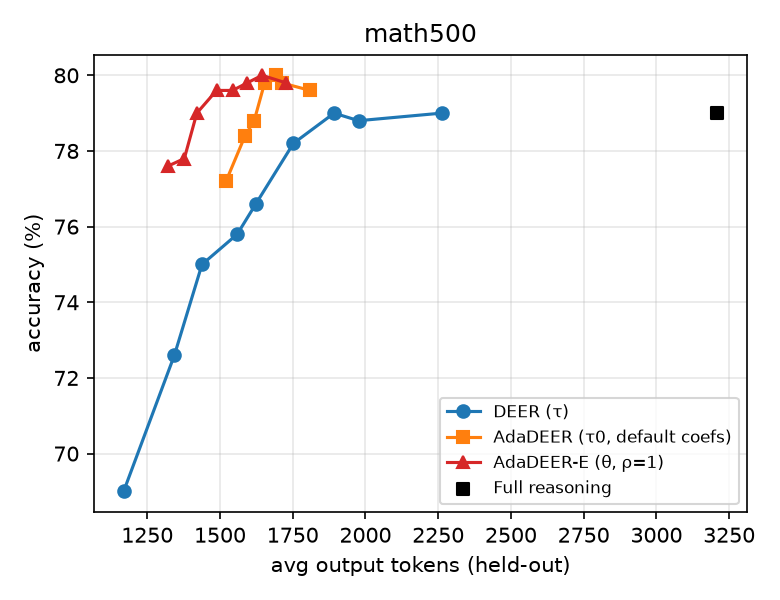
\includegraphics[width=\linewidth]{figures/math500_full_kfold_tradeoff.png}
\caption{MATH-500, 5-fold held-out means. AdaDEER-E (red) lies above the DEER threshold curve (blue) at every operating point near 1{,}300--1{,}700 tokens. Full reasoning (black square) is no more accurate and costs about twice the tokens.}
\label{fig:kfold}
\end{figure}

\begin{figure}[t]
\centering
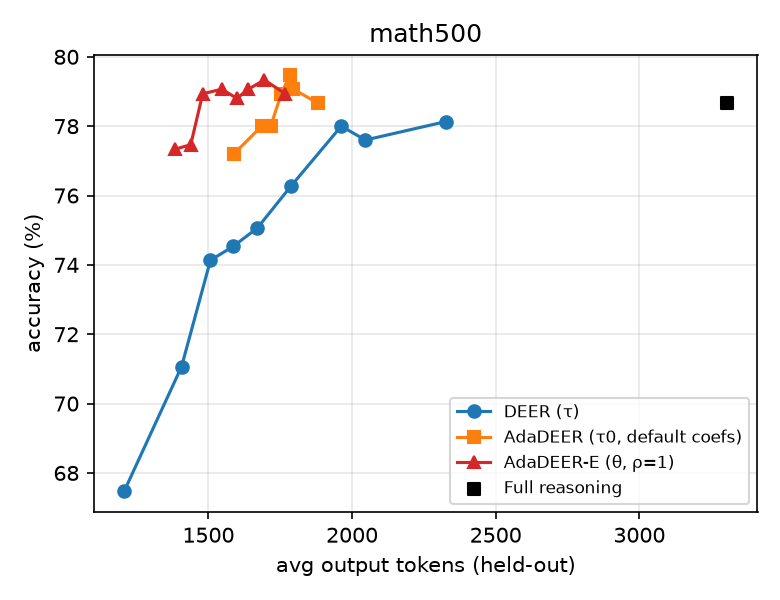
\includegraphics[width=\linewidth]{figures/math500_full_random_tradeoff.png}
\caption{The same comparison on five random 70/30 splits of all 500 MATH-500 problems. The red curve is again above the blue DEER curve. Iso-token gain of frozen AdaDEER-E on this protocol is $+4.7\pm 1.1$ points.}
\label{fig:random}
\end{figure}

Fig.~\ref{fig:kfold} and Fig.~\ref{fig:random} are the reason a single operating point is not enough.
Raising DEER's $\tau$ buys accuracy by delaying every exit, so the blue curve climbs and then flattens.
AdaDEER-E delays only unconfirmed exits.
Its red curve sits above that frontier: at a matched token budget the DEER curve is at 75.9\% while frozen AdaDEER-E is at 79.6\% on the 5-fold protocol ($+3.7\pm 2.5$ points), and at 74.4\% versus 79.1\% on the random splits ($+4.7\pm 1.1$ points).

\subsection{By difficulty}
Table~\ref{tab:level} breaks the 500 problems into MATH levels.
AdaDEER-E uses fewer tokens than DEER at $\tau=0.99$ at every level.
The largest saving is Level 5, 2{,}352 versus 3{,}112 tokens ($-24\%$), which is where a fixed high threshold waits the longest.
Accuracy is never below DEER at $\tau=0.95$.
Level sizes range from 43 to 134, so the Level 1 accuracy gap is a smaller sample than Level 5.

\begin{table}[t]
\caption{MATH-500 by difficulty, out of fold. Entries are accuracy / average tokens.}
\label{tab:level}
\centering
\footnotesize
\begin{tabular}{@{}lcccc@{}}
\toprule
Level & $n$ & DEER $0.95$ & DEER $0.99$ & AdaDEER-E \\
\midrule
1 & 43 & 90.7 / 769 & 93.0 / 853 & 93.0 / 632 \\
2 & 90 & 90.0 / 883 & 93.3 / 1{,}051 & 92.2 / 869 \\
3 & 105 & 85.7 / 1{,}194 & 86.7 / 1{,}374 & 90.5 / 1{,}147 \\
4 & 128 & 75.8 / 1{,}596 & 78.9 / 1{,}982 & 78.9 / 1{,}587 \\
5 & 134 & 56.7 / 2{,}756 & 59.0 / 3{,}112 & 59.0 / 2{,}352 \\
\bottomrule
\end{tabular}
\end{table}

\subsection{Ablation and tuning}
Table~\ref{tab:ablation} is the 5-fold mean on all 500 problems.
Tuned AdaDEER-E (79.4\% at 1{,}545 tokens) is not better than the frozen rule (79.6\% at 1{,}488).
The five training folds all choose $\theta=4.6$, and $\rho\in\{0.75,1\}$.
We therefore freeze rather than tune.
AdaDEER's default eight-parameter rule is 0.4 points more accurate and 14\% more expensive (1{,}694 versus 1{,}488 tokens).
The ablation says the extra parameters are not what produces the gain.

\begin{table}[t]
\caption{Component ablation on all 500 MATH-500 problems (5-fold mean). Tokens move when stability is removed and almost not otherwise.}
\label{tab:ablation}
\centering
\footnotesize
\begin{tabular}{@{}lcc@{}}
\toprule
Policy & Acc.\ (\%) & Tokens \\
\midrule
DEER $\tau=0.95$ & $76.6\pm 2.7$ & 1{,}623 \\
AdaDEER defaults & $80.0\pm 1.8$ & 1{,}694 \\
\quad no stability & $80.0\pm 2.8$ & 2{,}079 \\
\quad no volatility & $80.2\pm 2.0$ & 1{,}628 \\
\quad no switching & $80.2\pm 2.0$ & 1{,}675 \\
\quad no budget pressure & $80.0\pm 1.8$ & 1{,}704 \\
AdaDEER-E frozen & $79.6\pm 2.7$ & 1{,}488 \\
AdaDEER-E tuned & $79.4\pm 2.4$ & 1{,}545 \\
\bottomrule
\end{tabular}
\end{table}

\subsection{First 100 problems, and GSM8K}
On the first 100 problems of each set, with the same frozen parameters, AdaDEER-E is 85.0\% at 667 tokens on GSM8K (DEER $\tau=0.99$ is 85.0\% at 846) and 81.0\% at 1{,}345 tokens on MATH-500 (DEER $\tau=0.95$ is 79.0\% at 1{,}409; full reasoning is 81.0\% at 2{,}856).
Out of fold, AdaDEER-E is uniquely correct on 4 of these 200 problems and uniquely wrong on 1 (McNemar $p=0.375$).
With 100 problems per dataset the improvement is in the same direction as the 500-problem result and is not significant.
Fig.~\ref{fig:first100} is that smaller MATH-500 curve.
GSM8K accuracy matches DEER at $\tau=0.99$ with about 21\% fewer tokens (667 versus 846).
That is parity, not a significant accuracy gain.

\begin{figure}[t]
\centering
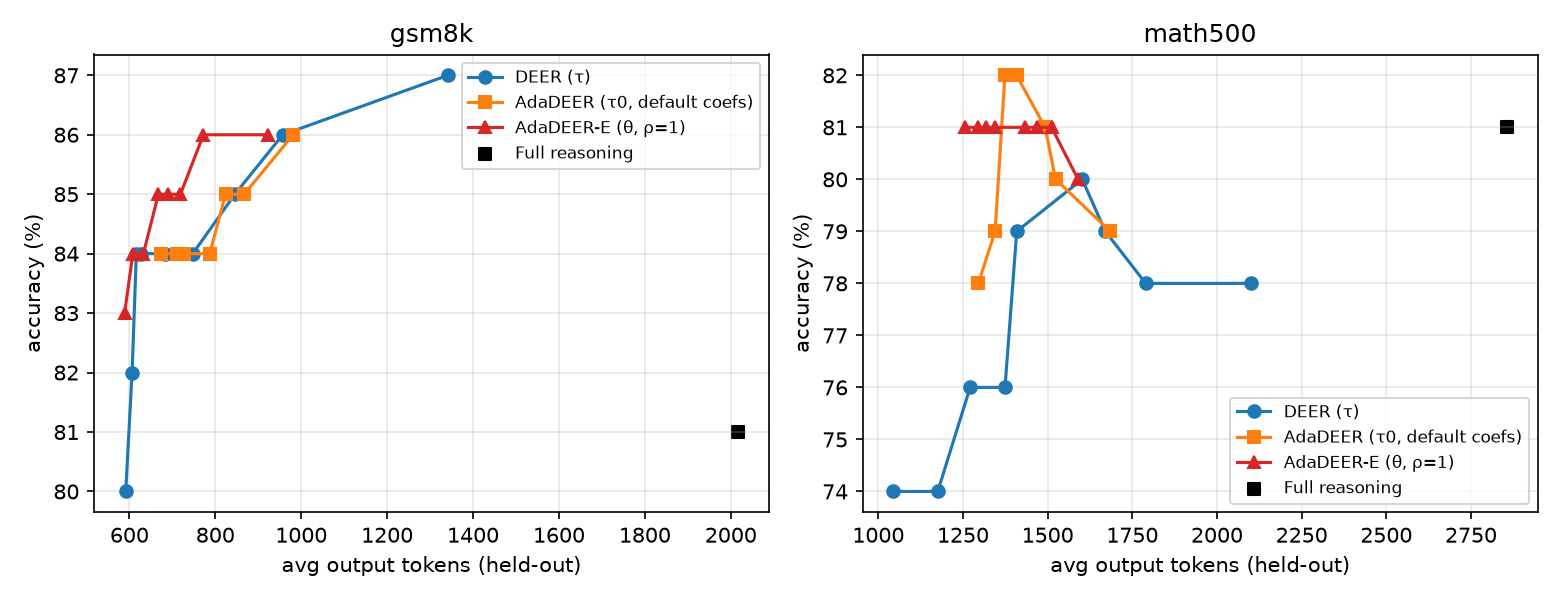
\includegraphics[width=\linewidth]{figures/first100_kfold_tradeoff.png}
\caption{First 100 MATH-500 problems, 5-fold means. The same frozen AdaDEER-E rule is at or above the DEER curve. Error bars across folds are large at this sample size, consistent with $p=0.375$ on the paired test.}
\label{fig:first100}
\end{figure}

\subsection{Why this rule, and not the neighbors}
Table~\ref{tab:decision} is the decision.
DEER at $0.95$ is cheaper than DEER at $0.99$ and less accurate.
DEER at $0.99$ matches full-reasoning accuracy by waiting on every problem.
A learned controller can beat raw confidence on GSM8K and does not on MATH-500, and it needs labels.
AdaDEER is the most accurate row and the one with the most knobs.
AdaDEER-E is the row that is simpler, frozen, significant against DEER at $0.95$, and no worse than DEER at $0.99$ while using fewer tokens.
$\rho=0$ returns DEER, so a bad setting of the new parameter is a setting we already know how to run.

\begin{table}[t]
\caption{What each stopping rule costs on all 500 MATH-500 problems.}
\label{tab:decision}
\centering
\footnotesize
\begin{tabular}{@{}lcccc@{}}
\toprule
 & Acc. & Tokens & Params & Train \\
\midrule
DEER $0.95$ & 76.6\% & 1{,}623 & 1 & no \\
DEER $0.99$ & 79.0\% & 1{,}892 & 1 & no \\
Learned controller & lower acc. & -- & many & yes \\
AdaDEER & 80.0\% & 1{,}694 & 8 & no \\
\textbf{AdaDEER-E} & \textbf{79.6\%} & \textbf{1{,}488} & \textbf{2} & \textbf{no} \\
\bottomrule
\end{tabular}
\end{table}

\section{Artifacts, Repository, and Check-Ins}
The repository is
{\scriptsize https://github.com/\allowbreak PeramVishnuSree/\allowbreak Adaptive-Early-Exit-for-\allowbreak Efficient-Reasoning-\allowbreak Reproducing-and-Extending-DEER}.
Table~\ref{tab:artifacts} points at the paths a reader needs.
The Overleaf source of this draft is \texttt{Jaswanthi Mandalapu/checkin4\_overleaf/main.tex}.
Upload that folder as an Overleaf project and compile \texttt{main.tex} with pdf\LaTeX.
Raw vLLM generation logs from the Check-In 3 and Check-In 4 live runs were written to Google Drive under \texttt{MyDrive/deer\_final/}.
A shareable Drive URL is not in the repository yet and has to be pasted here before the final submission.

\begin{table}[t]
\caption{Where the Check-In 4 artifacts live in the repository.}
\label{tab:artifacts}
\centering
\footnotesize
\begin{tabular}{@{}>{\raggedright\arraybackslash}p{0.46\linewidth}>{\raggedright\arraybackslash}p{0.48\linewidth}@{}}
\toprule
Path & Contents \\
\midrule
\path{Jaswanthi Mandalapu/Artifacts/adadeer/} &
AdaDEER-E policy, replay, grading, and the experiment driver. \\
\path{.../math500_full_kfold/} &
Table~\ref{tab:headline}, the ablation, and Fig.~\ref{fig:kfold}. \\
\path{.../math500_full_random/} &
70/30 splits of all 500 problems and Fig.~\ref{fig:random}. \\
\path{.../kfold/} and \path{random/} &
First 100 GSM8K and MATH-500, including Fig.~\ref{fig:first100}. \\
\path{.../traj/} &
Never-exit trajectories, including \path{full_math500.jsonl}. \\
\path{Vishnu-evaluation/} &
Live answer-fix runs and the stopping-method comparison. \\
\path{Saichetan-adaptive/} &
MLP controller and the state-dependent threshold note. \\
\bottomrule
\end{tabular}
\end{table}

Since the Check-In 3 snapshot on 2 November 2026, \texttt{main} contains these commits:
Vishnu Peram added training splits and the stopping-method comparison (three commits on 16 November);
Sai Chetan Muppalla added the state-dependent threshold and the held-out note;
and this check-in adds the AdaDEER-E code, the full MATH-500 replay, and this draft.
That is fewer than the 8--10 meaningful check-ins the assignment asks for after the previous check-in.
The count is stated as it is.
It should not be padded with empty commits.

The GitHub collaborators on this repository are the three authors.
The instructor and the TA are not on that list in the repository metadata this draft can see.
Check-In 3 said they had workspace access.
That invite still has to be confirmed on the GitHub repository and on the Drive folder before this draft is submitted.
This commit does not send invitations.

\section{Limitations}
The 500-problem numbers are an offline replay.
They answer ``which exit would this logged trajectory have taken,'' not ``what does a live AdaDEER-E generation emit.''
Check-In 3's simulator matched live DEER's exit on 100/100 GSM8K problems and 93/100 MATH-500 problems, which is why the replay is usable, and it is still not a live run.
The study uses one 1.5B model, greedy decoding, an 8{,}000-token budget, and two benchmarks.
The paper's own tables use a 16{,}000-token budget, so the absolute token counts are not a reproduction of those tables.
GSM8K in this replay has 100 problems, and the paired test is not significant.
The dev slice used to freeze $\theta$ and $\rho$ sits inside the 500; the dev-excluded cut is the mitigation, not a fully disjoint test set.
Check-In 3's state-dependent threshold (0.995 on the first checkpoint, 0.95 on a new answer, 0.85 on a repeat, and no exit on an unfinished formula) was shaped after reading misses on the same 200 problems, so that particular gain was optimistic.
AdaDEER-E does not use that rule.
Its parameters were frozen on the dev slice named above.
Check-In 2's synthetic accuracy figures are not results and are not repeated here.
Absolute GSM8K numbers differ between the vLLM logs and this MLX replay because the prompt and the checkpoint rate differ.
The two should not be averaged.

\section{Conclusion}
The project hypothesis from Check-In 1 holds, in a narrower form than the one we proposed.
A learned combination of trajectory features was not the part that beat a fixed threshold on MATH-500.
Confirmation was.
AdaDEER-E writes that fact as log-odds evidence: a new answer must clear $0.99$, a repeated answer accumulates, and an answer change resets the bar.
On all 500 MATH-500 problems the frozen rule is more accurate and cheaper than DEER at $\tau=0.95$, and as accurate as DEER at $\tau=0.99$ at 21\% fewer tokens, at under half the tokens of full reasoning.
The remaining work before the final submission, which this draft does not pretend is done, is a live run of the same rule, a shareable Drive link, invitations for the instructor and the TA, and enough further commits to meet the check-in count.

\begin{thebibliography}{9}
\bibitem{yang2025deer}
Y.~Yang \emph{et al.}, ``Dynamic early exit in reasoning models,'' in \emph{Proc.\ ICLR}, 2026, arXiv:2504.15895.
\bibitem{wei2022cot}
J.~Wei \emph{et al.}, ``Chain-of-thought prompting elicits reasoning in large language models,'' in \emph{Proc.\ NeurIPS}, 2022.
\bibitem{deepseekr1}
DeepSeek-AI, ``DeepSeek-R1: Incentivizing reasoning capability in LLMs via reinforcement learning,'' arXiv:2501.12948, 2025.
\bibitem{cobbe2021gsm8k}
K.~Cobbe \emph{et al.}, ``Training verifiers to solve math word problems,'' arXiv:2110.14168, 2021.
\bibitem{hendrycks2021math}
D.~Hendrycks \emph{et al.}, ``Measuring mathematical problem solving with the MATH dataset,'' in \emph{Proc.\ NeurIPS}, 2021.
\bibitem{checkin1}
J.~Mandalapu, S.~C.~Muppalla, and V.~S.~Peram, ``Adaptive early exit for efficient reasoning: Check-In 1,'' CMPE 258, San Jos\'{e} State University, 2026.
\bibitem{checkin2}
J.~Mandalapu, S.~C.~Muppalla, and V.~S.~Peram, ``Adaptive early exit for efficient reasoning: Check-In 2,'' CMPE 258, San Jos\'{e} State University, 2026.
\bibitem{checkin3}
J.~Mandalapu, S.~C.~Muppalla, and V.~S.~Peram, ``Adaptive early exit for efficient reasoning: Check-In 3,'' CMPE 258, San Jos\'{e} State University, 2026.
\end{thebibliography}

\end{document}
